\documentclass[a4paper]{article}
\usepackage{amssymb, amsmath}
\usepackage{graphicx}
\begin{document}
\section{Linear Regression}
\subsection{simple linear regression}
\begin{align*}
y = \beta_1 + \beta_2 x + \epsilon
\end{align*}
{\bf Assumptions}\\
1. Linear \\
2. X matrix is fixed.\\
3. error term has zero mean\\
4. Homescedasticity or equal variance of $\epsilon$\\
5. No autocorrelation between disturbances.$cov(\epsilon_i, \epsilon_j)=0$.\\
6. Zero covariance between $\epsilon_i, X_i$.\\
7. Number of obsearvations n must be greater than the number of parameters.\\
8. $Var(X) > 0$.\\
9. no multicollinearity.\\
\begin{align*}
Y = X{\boldsymbol \beta} + \epsilon
\end{align*}
Where Y is a nx1 matrix, X is anxp matrix, beta is px1 vector and $\epsilon$ is nx1 vector with $\epsilon_i$ begin iid with normal distribution
\subsection{Least Square Regression Model}
The cost function is given by
\begin{align*}
f(\boldsymbol \beta) = ||Y-X\beta||^2 & = (Y-X\beta)^T(Y-X\beta)
                      & = Y^T Y - Y^TX\beta - \beta^TX^TY +\beta^TX^T X \beta
\end{align*}
Since third term are scalar, 
\begin{align*}
 \beta^TX^TY = (\beta^TX^TY)^T = Y^TX\beta 
\end{align*}
\begin{align*}
f(\beta) = Y^T Y - 2Y^TX\beta - \beta^TX^T X \beta
            = Y^T Y - 2(X^TY)^T\beta + \beta^TX^T X \beta
\end{align*}
The first term is a constant and its derivative is zero. \\
{\bf The deriviative of 2nd term}\\
Consider the derivative of $\alpha^T \beta$ with respect to $\beta$.
\begin{align*}
\boldsymbol{\alpha}^T \boldsymbol{\beta} = \Sigma \alpha_i \beta_i \\
\frac{\partial{\boldsymbol{\alpha}^T\boldsymbol{\beta}}}{\partial \beta_i} = \alpha_i\\
\end{align*}
Write the derivative in matrix form
\begin{align*}
\left(  \begin{array} {c}
		\frac{\partial{\boldsymbol{\alpha}^T\boldsymbol{\beta}}}{\partial \beta_1}\\
		\frac{\partial{\boldsymbol{\alpha}^T \boldsymbol{\beta}}}{\partial \beta_2}\\
                  ...\\
		\frac{\partial{\boldsymbol{\alpha}^T \boldsymbol{\beta}}}{\partial \beta_3}\\
		\end{array}
		\right) 
=\left(  \begin{array} {c}
		\alpha_1\\
		\alpha_2\\
                  ...\\
		\alpha_p\\
		\end{array}
		\right) 
\end{align*}
So if we let $\alpha= X^TY$, we have
\begin{align*}
\frac{\partial{2(X^TY)^T\beta}}{\partial \beta} = 2X^TY
\end{align*}
{\bf The derivative of 3rd term}\\
let $A=X^TX$,
\begin{align*}
\beta^TX^T X \beta = \beta^T
\left(  \begin{array} {c}
		\Sigma_i A_{1k}\beta_{k}\\
		 \Sigma_i A_{2k}\beta_{k}\\
                  ...\\
		 \Sigma_k A_{pk}\beta_{k}\\
		\end{array}
		\right) 
 =  \Sigma_j \beta_j (\Sigma_k A_{jk}\beta_k)
\end{align*}
To calculate the derivative of $f(\beta)$, we note there are only 3 cases that the derivative does not vanish\\
1) l = j = k 
\begin{align*}
\frac{f(\boldsymbol \beta)}{\partial \beta_l} 
= 2 A_{ll} \beta_l 
\end{align*}
2) l=j, j $\neq$ k
\begin{align*}
\frac{f(\boldsymbol \beta)}{\partial \beta_l} 
= \Sigma_{k, k\neq l} A_{lk}\beta_{k}\\
\end{align*}
3) l=k, j $\neq$ k
\begin{align*}
\frac{f(\boldsymbol \beta)}{\partial \beta_l} 
= \Sigma_{j, j\neq l} A_{jl}\beta_{j} = \Sigma_{j,  j\neq l} A^T_{lj}\beta{j}
\end{align*}
Therefore
\begin{align*}
\frac{f(\boldsymbol \beta)}{\partial \beta_l}  = A_{ll} \beta_l + \Sigma_{k, k\neq l} A_{lk}\beta_{k} + A_{ll} \beta_l + \Sigma_{j, j \neq l} A^T_{lj}\beta{j} \\
= \Sigma_{k} A_{lk}\beta_{k} + \Sigma_{j} A^T_{lj}\beta{j}
\end{align*}
The first term is the lth row of vector $A\beta = X^TX\beta$, and the 2nd term is the lth row of vector$A^T\beta=X^TX\beta$. So we put the whole derivative in matrix form
\begin{align*}
\frac{f(\boldsymbol \beta)}{\partial {\boldsymbol \beta}} = -2X^TY+2X^TX\beta
\end{align*}
which is a px1 vector with each row corresponding to the derivative with respect to $\beta_i$
letting the derivative equal to zero yields the estimation of $\beta$
\begin{align*}
\hat \beta = (X^TX)^{-1}X^TY
\end{align*}
\subsection{Least Square Estimator for Simple Linear Regression}
\begin{align*}
	&\left(  \begin{array} {c}
		\beta_{0} \\
		\beta_{1} \\
		\end{array}
		\right) \\
=& (X^TX)^{-1}X^TY \\
=&\left( \left(  \begin{array} {cccc}
		1 & 1 &... &1\\
		x_1 & x_2 &... &x_n \\
		\end{array}
		\right) 
    \left(  \begin{array} {cc}
		1 & x_1 \\
		1 & x_2 \\
                   1 & x_n \\
		\end{array}
		\right) 
\right)^{-1}
\left(  \begin{array} {cccc}
		1 & 1 &... &1\\
		x_1 & x_2 &... &x_n \\
		\end{array}
		\right) 
\left(  \begin{array} {c}
		y_1 \\
		y_2 \\
                  ... \\
                  y_n
		\end{array}
		\right) \\
=& \frac{1}{n\Sigma x^2_i - (\Sigma x_i)^2}
\left(  \begin{array} {cc}
	          \Sigma_i x_i^2 & -\Sigma_i x_i \\
		 -\Sigma_i x_i &n\\
		\end{array}
		\right) 
\left(  \begin{array} {c}
	          \Sigma_i y_i \\
		 -\Sigma x_i y_i\\
		\end{array}
		\right) 
\end{align*}
So
\begin{align*}
\beta_1 = \frac{\Sigma x_i^2 \Sigma y_i - \Sigma x_i (\Sigma x_i y_i)}{n\Sigma x^2_i - (\Sigma x_i)^2} \\
\beta_2 = \frac{-\Sigma x_i \Sigma y_i + n \Sigma x_i y_i}{n\Sigma x^2_i - (\Sigma x_i)^2}
\end{align*}
\subsection{Projection matrix}
Given $\hat \beta = (X^TX)^{-1}X^TY$, we have the predictor value of $y=X\beta$ 
\begin{align*}
\hat y = X(X^TX)^{-1}X^T y
\end{align*}
The matrix $P=X(X^TX)^{-1}X^T$ is a projection matrix. It projects the vector of y into the column space of X.\\
{\bf Understand the word projection}\\
Let us understand this first through geometry point of view. Consider a vector on 2 dimensional space, $V_1= (x_1, y_1)^T$, where $x_1$ and $y_1$ are the x and y component, respectively. If we project the vector V into x-line, then apparently we get $V_x= (x_1, 0)^T$, see graph below.

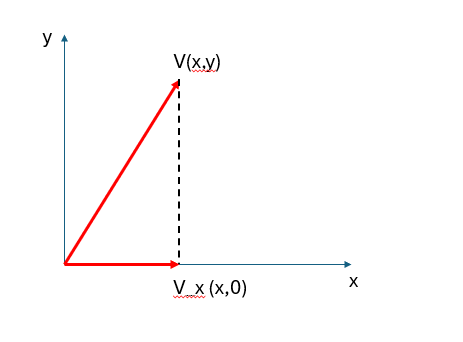
\includegraphics[scale = 1]{project1.png}\\
If we have a vector that is along the x axis
\begin{align*}
X = \left( \begin{array} {c }
              1  \\
              0  \\
            \end{array} \right)\\
\end{align*}
 The projection matrix of a vector into x line is 
\begin{align*}
P_x & = x(x^Tx)^{-1}x^T \\
     & = \left( \begin{array} {c}
              1 \\
              0 \\
            \end{array} \right)
 \left( \begin{array} { c  c } 
                   1 & 0\\
           \end{array} \right) \\
       & =  \left( \begin{array} { c  c } 
                   1 & 0  \\
                   0 & 0  \\
           \end{array} \right)
\end{align*}
Applying this projection matrix to any 2 dimensional vector $V$ gives $(V_x, 0)^T$. So it projects the vector into x line. 
Let us take another example. Imagine $V_1$ is vector if we project $V$ onto the line that has 45 degree angle with x axis. See below.

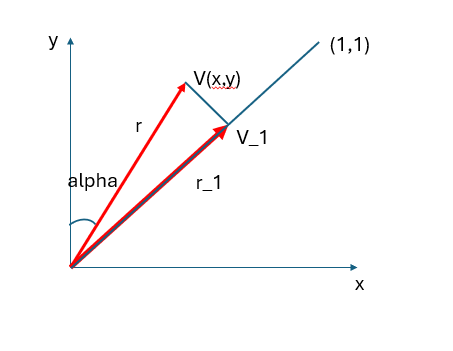
\includegraphics[scale = 1]{project2.png}\\

In order to calculate $V_1$,  we see
\begin{align*}
r_1 = r cos(\pi/4 - alpha) =r( \frac{\sqrt{2}}{2} \frac{y}{r} + \frac{\sqrt{2}}{2} \frac{x}{r}) = \frac{\sqrt 2}{2}y +\frac{\sqrt2}{2} x
\end{align*}
\begin{align*}
V_{1x}=r_1cos(\pi/4)=\frac{x+y}{2}\\
V_{1y}=r_1sin(\pi/4)=\frac{x+y}{2}\\
\end{align*}
After we understand this using geometry point of view, we can workout from algebra point of view. The vector we want to project onto is
\begin{align*}
i = \left( \begin{array} {c }
              1  \\
              1  \\
            \end{array} \right)\\
\end{align*}
The projection matrix of a vector into x line is 
\begin{align*}
P_x & = x(x^Tx)^{-1}x^T \\
     & = \left( \begin{array} {c}
              1 \\
              1 \\
            \end{array} \right)
\left( \left( \begin{array} {c c}
              1 & 1\\
            \end{array} \right) 
          \left( \begin{array} {c }
              1 \\
              1 \\
            \end{array} \right) \right)^{-1}
 \left( \begin{array} { c  c } 
                   1 & 1\\
           \end{array} \right) \\
       & =  \frac{1}{2}\left( \begin{array} { c  c } 
                   1 & 1  \\
                   1 & 1  \\
           \end{array} \right)
\end{align*}
Therefore we easily see
\begin{align*}
V_1 =  \frac{1}{2}\left( \begin{array} { c  c } 
                   1 & 1  \\
                   1 & 1  \\
           \end{array} \right) 
             \left( \begin{array} {c }
              x \\
              y \\
            \end{array} \right)
          = \left( \begin{array} {c }
              \frac{1}{2} (x+y) \\
              \frac{1}{2} (x+y) \\
            \end{array} \right)
\end{align*}
which is the same as what we get based on geometry.
 For n dimensional vector y, if our X matrix has rank of k, then the projection matrix P projects the vector y into k dimensional hyperplane. For example, if we define
\begin{align*}
i_N =   \left( \begin{array} {c }
              1 \\
              1 \\
             ...\\
              1
            \end{array} \right)
\end{align*}
The projection matrix P is
\begin{align*}
P = i \frac{1}{N}i^T
  = \frac{1}{N} \left( \begin{array} { c  c c c } 
                   1 & 1 & ... & 1 \\
                   1 & 1 & ... & 1 \\
                   ... & ... & ... & ... \\
                   1 & 1 & ... & 1 \\
           \end{array} \right) 
\end{align*}
{\bf Projection matrix into null space}\\
If $P$ is a projection matrix, the matrix $I - P$ is also a projection matrix. In linear regression model
\begin{align*}
y &= X\beta +\epsilon\\
P &= X(X^TX)^{-1}X^T\\
\hat \epsilon & = (I - P) y = (I - X(X^TX)^{-1}X^T)y\\
\end{align*}
For the above example, we define $M = I - \frac{1}{N}i i^T$, and $My$ express the mean deviations of a vector.\\
{\bf Idempotent property of projection matrix\\}
Consider the previous example that we project a vector V onto x axis, how about we do this projection twice, we would end up the same vector $V_x$. Using a little matrix algebra, it is easy to prove that for any project matrix P, we have $PP=P$.  
\subsection{Variance of $\hat \beta$}
\begin{align*}
Var(\hat \beta)
=Var((X^TX)^{-1}X^T \epsilon)
=(X^TX)^{-1}X^T Var( \epsilon) ((X^TX)^{-1}X^T)^T\\
=\sigma^2 (X^TX)^{-1}X^T  X (X^TX)^{-1}
=\sigma^2 (X^TX)^{-1}
\end{align*}
For simple linear regression
\begin{align*}
Var(\hat \beta)
=\frac{\sigma^2}{n\Sigma x_i^2 - (\Sigma x_i)^2} \left(  \begin{array} {cc}
	          \Sigma_i x_i^2 & -\Sigma_i x_i \\
		 -\Sigma_i x_i &n\\
		\end{array}
		\right) 
\end{align*}
\begin{align*}
Var(\hat \beta_1) =\frac{\Sigma x_i^2 \sigma^2}{n\Sigma x_i^2 - (\Sigma x_i)^2} 
\end{align*}
\begin{align*}
Var(\hat \beta_2) =\frac{n \sigma^2}{n\Sigma x_i^2 - (\Sigma x_i)^2} 
\end{align*}
Try
\begin{align*}
\Sigma (x_i- \bar x)^2 = \Sigma(x_i^2 - 2 \bar x x_i+ \bar x^2)
= \Sigma_i(x_i^2 - 2 (\Sigma_j \frac{x_j}{n}) x_i + \frac{ (\Sigma_j x_j)^2} {n^2})\\
=\Sigma_ix_i^2 - \frac{2}{n} (\Sigma_i x_i)^2 + \frac{ (\Sigma_i x_i)^2} {n}
= \Sigma_i x^2_i - \frac{1}{n} (\Sigma x_i)^2
\end{align*}
So
\begin{align*}
Var(\hat \beta_1) =\frac{\Sigma x_i^2 \sigma^2}{n\Sigma (x_i- \bar x)^2 } 
\end{align*}
\begin{align*}
Var(\hat \beta_2) =\frac{n \sigma^2}{n\Sigma (x_i- \bar x)^2} = \frac{\sigma^2}{\Sigma (x_i- \bar x)^2}
\end{align*}
\subsection{Sum of Square Error}
\begin{align*}
SSE
&=\Sigma_i (y-\hat y_i)^2 \\
& = (Y-X\beta)^T(Y-X\beta) \\
& = (Y-X(X^TX)^{-1}X^TY)^T(Y-X(XTX)-1X^TY) \\
& = (Y-PY)^T(Y-PY) \\
& = Y^T(1-P)^T(1-P)Y = Y^T(1-P)Y \\
& = (X\beta + \epsilon) ^T (1-P)(X\beta+\epsilon) \\
& = \beta^T X^T (1-P)X\beta + 2\beta^T X^T X^T(I-P)\epsilon 
   + \epsilon^T(I-H)\epsilon 
\end{align*}
\begin{align*}
E[SSE] = E[\epsilon^T(I-P)\epsilon] = E[\epsilon^T \epsilon] trace(I-H)
          = \sigma^2(n-p)\\
\end{align*}

\end{document}